\documentclass{article}
% Change "article" to "report" to get rid of page number on title page
\usepackage{amsmath,amsfonts,amsthm,amssymb}
\usepackage{setspace}
\usepackage{upgreek}
\usepackage{Tabbing}
\usepackage{fancyhdr}
\usepackage[utf8]{inputenc}

\usepackage{lastpage}
\usepackage{extramarks}
\usepackage{chngpage}
\usepackage{soul,color}
\usepackage{tikz}
\usetikzlibrary{arrows,automata}
\usetikzlibrary{shapes.arrows,chains,positioning}
\usepackage{fancybox}
\usepackage{graphicx,float,wrapfig}

% In case you need to adjust margins:
\topmargin=-0.45in      %
\evensidemargin=0in     %
\oddsidemargin=0in      %
\textwidth=6.5in        %
\textheight=9.0in       %
\headsep=0.25in         %

% Homework Specific Information
\newcommand{\hmwkTitle}{Tarea \#3}
\newcommand{\hmwkDueDate}{Lunes,\ Marzo\ 8,\ 2010}
\newcommand{\hmwkClass}{CC3006}
\newcommand{\hmwkClassTime}{}
\newcommand{\hmwkClassInstructor}{Bidkar Pojoy}
\newcommand{\hmwkAuthorName}{Carlos E. L\'{o}pez Camey}


\newcommand{\set}[1]{\{ #1  \}}
\newcommand{\cerradura}[1]{cerradura$-$\epsilon(#1) }


% Setup the header and footer
\pagestyle{fancy}                                                       %
\lhead{\hmwkAuthorName}                                                 %
\chead{\hmwkClass\ (\hmwkClassInstructor\ \hmwkClassTime): \hmwkTitle}  %
\rhead{\firstxmark}                                                     %
\lfoot{\lastxmark}                                                      %
\cfoot{}                                                                %
\rfoot{Page\ \thepage\ of\ \pageref{LastPage}}                          %
\renewcommand\headrulewidth{0.4pt}                                      %
\renewcommand\footrulewidth{0.4pt}                                      %

% This is used to trace down (pin point) problems
% in latexing a document:
%\tracingall

%%%%%%%%%%%%%%%%%%%%%%%%%%%%%%%%%%%%%%%%%%%%%%%%%%%%%%%%%%%%%
% Some tools
%\newcommand{\enterProblemHeader}[1]{\nobreak\extramarks{#1}{#1 continued on next page\ldots}\nobreak%
   %                                 \nobreak\extramarks{#1 (continued)}{#1 continued on next page\ldots}\nobreak}%
\newcommand{\exitProblemHeader}[1]{\nobreak\extramarks{#1 (continued)}{#1 continued on next page\ldots}\nobreak%
                                   \nobreak\extramarks{#1}{}\nobreak}%

\newlength{\labelLength}
\newcommand{\labelAnswer}[2]
  {\settowidth{\labelLength}{#1}%
   \addtolength{\labelLength}{0.25in}%
   \changetext{}{-\labelLength}{}{}{}%
   \noindent\fbox{\begin{minipage}[c]{\columnwidth}#2\end{minipage}}%
   \marginpar{\fbox{#1}}%

   % We put the blank space above in order to make sure this
   % \marginpar gets correctly placed.
   \changetext{}{+\labelLength}{}{}{}}%

\setcounter{secnumdepth}{0}
\newcommand{\homeworkProblemName}{}%
\newcounter{homeworkProblemCounter}%
\newenvironment{homeworkProblem}[1][Problem \arabic{homeworkProblemCounter}]%
  {\stepcounter{homeworkProblemCounter}%
   \renewcommand{\homeworkProblemName}{#1}%
   \section{\homeworkProblemName}%
   %\enterProblemHeader{\homeworkProblemName}
   }%
  %{\exitProblemHeader{\homeworkProblemName}}%

\newcommand{\problemAnswer}[1]
  {\noindent\fbox{\begin{minipage}[c]{\columnwidth}#1\end{minipage}}}%

\newcommand{\problemLAnswer}[1]
  {\labelAnswer{\homeworkProblemName}{#1}}

\newcommand{\homeworkSectionName}{}%
\newlength{\homeworkSectionLabelLength}{}%
\newenvironment{homeworkSection}[1]%
  {% We put this space here to make sure we're not connected to the above.
   % Otherwise the changetext can do funny things to the other margin

   \renewcommand{\homeworkSectionName}{#1}%
   \settowidth{\homeworkSectionLabelLength}{\homeworkSectionName}%
   \addtolength{\homeworkSectionLabelLength}{0.25in}%
   \changetext{}{-\homeworkSectionLabelLength}{}{}{}%
   \subsection{\homeworkSectionName}%
   \enterProblemHeader{\homeworkProblemName\ [\homeworkSectionName]}}%
  {\enterProblemHeader{\homeworkProblemName}%

   % We put the blank space above in order to make sure this margin
   % change doesn't happen too soon (otherwise \sectionAnswer's can
   % get ugly about their \marginpar placement.
   \changetext{}{+\homeworkSectionLabelLength}{}{}{}}%

\newcommand{\sectionAnswer}[1]
  {% We put this space here to make sure we're disconnected from the previous
   % passage

   \noindent\fbox{\begin{minipage}[c]{\columnwidth}#1\end{minipage}}%
   \enterProblemHeader{\homeworkProblemName}\exitProblemHeader{\homeworkProblemName}%
   \marginpar{\fbox{\homeworkSectionName}}%

   % We put the blank space above in order to make sure this
   % \marginpar gets correctly placed.
   }%

%%%%%%%%%%%%%%%%%%%%%%%%%%%%%%%%%%%%%%%%%%%%%%%%%%%%%%%%%%%%%


%%%%%%%%%%%%%%%%%%%%%%%%%%%%%%%%%%%%%%%%%%%%%%%%%%%%%%%%%%%%%
% Make title
\title{\textmd{\textbf{\hmwkClass:\ \hmwkTitle}}\\\normalsize\vspace{0.1in}\small{Para entregar\ el\ \hmwkDueDate}\\\vspace{0.1in}\large{\textit{\hmwkClassInstructor\ \hmwkClassTime}}}
\date{}
\author{\textbf{\hmwkAuthorName}}
%%%%%%%%%%%%%%%%%%%%%%%%%%%%%%%%%%%%%%%%%%%%%%%%%%%%%%%%%%%%%

\begin{document}
\begin{spacing}{1.1}
\maketitle
% Uncomment the \tableofcontents and \newpage lines to get a Contents page
% Uncomment the \setcounter line as well if you do NOT want subsections
%       listed in Contents
%\setcounter{tocdepth}{1}
%\tableofcontents


%\newpage

% When problems are long, it may be desirable to put a \newpage or a
% \clearpage before each homeworkProblem environment
\begin{homeworkProblem}[Construya un AFN a partir de la expresi\'{o}n regular con el algoritmo de \textbf{Construcci\'{o}n de Thompson}]

% (a*|b*)c
\subsection{1. (a*$|$b*)c}

\begin{center}
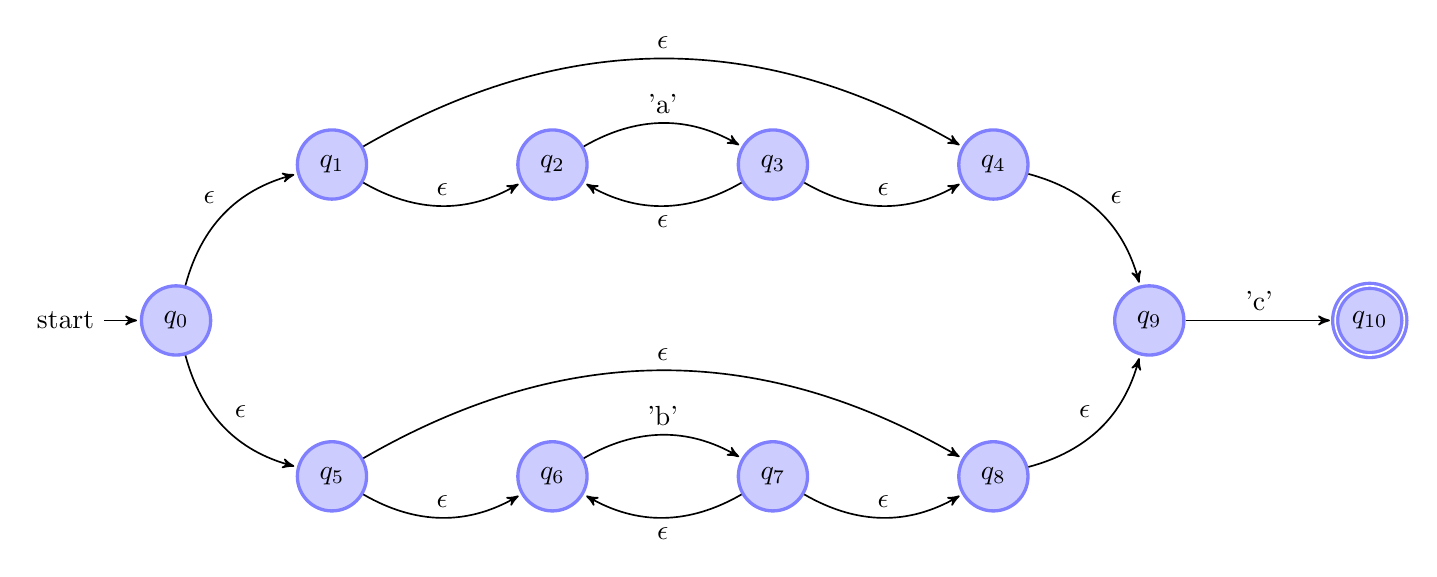
\begin{tikzpicture}[->,>=stealth',shorten >=1pt,auto,node distance=2.8cm,semithick]
  \tikzstyle{every state}=[draw=blue!50,very thick,fill=blue!20]

  \node[initial,state] 	(q0)                   			 {$q_0$};
  % kleene(a)
  \node[state]		(q1)	[above right of =q0]	 {$q_1$};
  \node[state]		(q2)	[right of =q1]	 {$q_2$};
  \node[state]		(q3)	[right of =q2]	 {$q_3$};  
  \node[state]		(q4)	[right of =q3]	 {$q_4$};  
  %kleene(b)
  \node[state]		(q5)	[below right of =q0]	{$q_5$};
  \node[state]		(q6)	[right of =q5]	 {$q_6$};
  \node[state]		(q7)	[right of =q6]	 {$q_7$};  
  \node[state]		(q8)	[right of =q7]	 {$q_8$};  
  %final state from a*|b*
  \node[state]		(q9)	[below right of =q4]	 {$q_9$};  
  \node[state,accepting] (q10)[right of =q9]		{$q_{10}$};
		
  \path 			%a*|b*
  				(q0)	edge		[bend left]		node {$\epsilon$}	(q1)
				(q0)	edge		[bend right]	node {$\epsilon$}	(q5)
				% a*
				(q1)  edge		[bend right]	node {$\epsilon$}	(q2)
				(q1)  edge		[bend left]		node {$\epsilon$}	(q4)
				(q3)  edge		[bend left]		node {$\epsilon$}	(q2)
				(q2)  edge		[bend left]		node {'a'}	(q3)
				(q3)  edge		[bend right]	node {$\epsilon$}	(q4)
				%b*				
				(q5)  edge		[bend right]	node {$\epsilon$}	(q6)
				(q5)  edge		[bend left]		node {$\epsilon$}	(q8)
				(q7)  edge		[bend left]		node {$\epsilon$}	(q6)
				(q6)  edge		[bend left]		node {'b'}	(q7)
				(q7)  edge		[bend right]		node {$\epsilon$}	(q8)
				%end a* | b*
				(q4)  edge		[bend left]		node {$\epsilon$}	(q9)
				(q8)  edge		[bend right]	node {$\epsilon$}	(q9)
				%end concatenation 
				(q9)	edge					node {'c'}	(q10);
\end{tikzpicture}
\end{center}

\section{Convierta el AFN resultante a un AFD que reconozca el mismo lenguaje con el algoritmo de \textbf{Construcci\'{o}n de sub-conjuntos}}

$q_a = cerradura$-$\epsilon(q_0) = \set{q_0,q_1,q_2,q_4,q_5,q_6,q_8,q_9} = A$ \\
$Q = \set{A}$\\
$marcados = \set{}$\\
$\delta= \set{}$\\
\indent $marcados = \set{A}$ \\
\indent \indent para 'a' \\
\indent \indent \indent $U = \cerradura{mueve(A,a) } = \set{q_3,q_2,q_4,q_9} = B$ \\
\indent \indent \indent $Q = \set{A,B}$\\
\indent \indent \indent $\delta = \set{(A,a) -> B}$ \\
\indent \indent para 'b'\\
\indent \indent \indent $U = \cerradura{mueve(A,b) } = \set{q_6,q_7,q_8,q_9} = C$ \\
\indent \indent \indent $Q = \set{A,B,C}$\\
\indent \indent \indent $\delta = \set{(A,a) -> B,(A,b) -> C}$\\
\indent \indent para 'c' \\
\indent \indent \indent $U = \cerradura{mueve(A,c) } = \set{q_{10}} = D$ \\
\indent \indent \indent $Q = \set{A,B,C,D}$\\
\indent \indent \indent $\delta = \set{(A,a) -> B,(A,b) -> C,(A,c) -> D}$\\

\indent $marcados = \set{A,B}$\\
\indent \indent para 'a' \\
\indent \indent \indent $U = \cerradura{mueve(B,a) } = \set{q_3,q_2,q_4,q_9} = B$ \\
\indent \indent \indent $\delta = \set{(A,a) -> B,(A,b) -> C,(A,c) -> D,(B,a) -> B}$\\
\indent \indent para 'b'\\
\indent \indent \indent $U = \set{} $\\
\indent \indent para 'c' \\
\indent \indent \indent $U = \cerradura{mueve(B,c) } = \set{q_{10}} = D$ \\
\indent \indent \indent $\delta = \set{(A,a) -> B,(A,b) -> C,(A,c) -> D,(B,a) -> B, (B,c) -> D}$\\

\indent $marcados = \set{A,B,C}$\\
\indent \indent para 'a' \\
\indent \indent \indent $U = \set{}$ \\
\indent \indent para 'b'\\
\indent \indent \indent $U = \cerradura{mueve(C,b) } = \set{q_6,q_7,q_8,q_9} = C $\\
\indent \indent \indent $\delta = \set{(A,a) -> B,(A,b) -> C,(A,c) -> D,(B,a) -> B, (B,c) -> D,(C,b) -> C}$\\
\indent \indent para 'c' \\
\indent \indent \indent $U = \cerradura{mueve(C,c) } = \set{q_{10}} = D$ \\
\indent \indent \indent $\delta = \set{(A,a) -> B,(A,b) -> C,(A,c) -> D,(B,a) -> B, (B,c) -> D,(C,b) -> C,(C,c) -> D}$\\

\indent $marcados = \set{A,B,C,D}$\\
\indent \indent para 'a' \\
\indent \indent \indent $U = \set{}$ \\
\indent \indent para 'b'\\
\indent \indent \indent $U = \set{}$\\
\indent \indent para 'c' \\
\indent \indent \indent $U = \set{}$ \\

\subsection{AFD con Construcci\'{o}n de Sub-conjuntos:}
\begin{center}
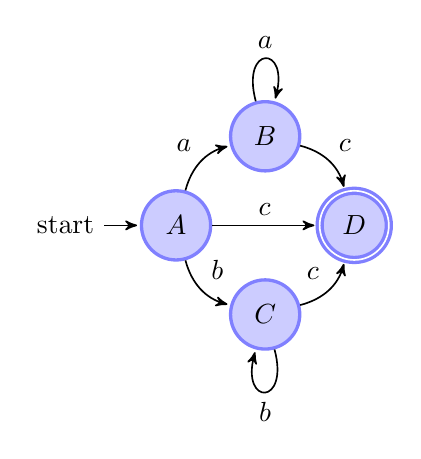
\begin{tikzpicture}[->,>=stealth',shorten >=1pt,auto,node distance=1.6cm,semithick]
  \tikzstyle{every state}=[draw=blue!50,very thick,fill=blue!20]

  \node[initial,state] 	(A)                   			 {$A$};
  % kleene(a)
  \node[state]		(B)	[above right of =A]	 {$B$};
  \node[state]		(C)	[below right of =A]	 {$C$};
    \node[state,accepting]		(D)	[above right of =C]	 {$D$};
 
		
  \path 			(A)	edge		[bend left]		node {$a$}	(B)
  					edge		[bend right]	node{$b$}	(C)
					edge					node{$c$}		(D)
				(B)	edge		[loop above]	node{$a$}	(B)
					edge		[bend left]		node{$c$}		(D)
				(C)	edge		[loop below]	node{$b$}	(C)
					edge		[bend right]	node{$c$}		(D);
\end{tikzpicture}
\end{center}

\section{Construya directamente un AFD que reconozca el lenguaje generado por la expresi\'{o}n regular}

\begin{center}
\begin{tikzpicture}[level/.style={sibling distance=100mm/#1}]
\node (root) {$\cdot$} 
	child {node {$\cdot$}
		child {node {$|$}
			child {node {*}
				child {node {$a$}}
			}					 
			child {node {*}
				child {node {$b$}}
			}			
		} 
		child {node {$c$}}
	}
	child {node {\#}}
	;
	
	%positions
	\node[below right of=root-2]  {$p = 4$};
	\node[below right of=root-1-2]  {$p = 3$};
	\node[below right of=root-1-1-1-1]  {$p= 1$};
	\node[below right of=root-1-1-2-1]  {$p=2$};
	
	%primerapos
	\node[left of=root]  {$\set{1,2,3}$};
	\node[left of=root-1]  {$\set{1,2,3}$};	
	\node[left of=root-2]  {$\set{4}$};
	\node[left of=root-1-1]  {$\set{1,2}$};
	\node[left of=root-1-2]  {$\set{3}$};
	\node[left of=root-1-1-1]  {$\set{1}$};
	\node[left of=root-1-1-2]  {$\set{2}$};
	\node[left of=root-1-1-1-1]  {$\set{1}$};
	\node[left of=root-1-1-2-1]  {$\set{2}$};
	
	%ultimapos
	\node[right of=root]  {$\set{4}$};
	\node[right of=root-1]  {$\set{3}$};
	\node[right of=root-2]  {$\set{4}$};
	\node[right of=root-1-1]  {$\set{2}$};
	\node[right of=root-1-2]  {$\set{3}$};
	\node[right of=root-1-1-1]  {$\set{1}$};
	\node[right of=root-1-1-2]  {$\set{2}$};
	\node[right of=root-1-1-1-1]  {$\set{1}$};
	\node[right of=root-1-1-2-1]  {$\set{2}$};
	%\draw (root-1.center) -- node[above,sloped] {sibling distance} (root-2.center);		
\end{tikzpicture}

\begin{tabular}{ l r }
  $p$ & $siguientePos$\\
\hline
  1 &  3,1 \\
  2 &  3,2 \\
  3 &  4 \\
\end{tabular}
\end{center}


$q_0 = \set{1,2,3}$ \\
$Q = \set{A}$ \\
$\delta = \set{}$ \\
\indent $marcados = \set{A}$\\
\indent \indent para 'a' \\
\indent \indent \indent $ v = sigPos(1) = \set{1,3} = B$ \\
\indent \indent \indent $Q = \set{A,B}$ \\
\indent \indent \indent $\delta = \set{(A,a) -> B}$ \\
\indent \indent para 'b' \\
\indent \indent \indent $ v = sigPos(2) = \set{2,3} = C$\\ 
\indent \indent \indent $Q = \set{A,B,C}$\\
\indent \indent \indent $\delta = \set{(A,a) -> B, (A,b) -> C}$\\
\indent \indent para 'c'\\
\indent \indent \indent $ v = sigPos(3) = \set{4} = D$\\
\indent \indent \indent $Q = \set{A,B,C,D}$\\
\indent \indent \indent $\delta = \set{(A,a) -> B, (A,b) -> C, (A,c) -> D}$\\

\indent $marcados = \set{A,B}$\\
\indent \indent para 'a' \\
\indent \indent \indent $ v = sigPos(1) = \set{1,3} = B$ \\
\indent \indent \indent $\delta = \set{(A,a) -> B, (A,b) -> C, (A,c) -> D,(B,a) -> B}$\\
\indent \indent para 'b' \\
\indent \indent \indent $ v = \set{}$\\ 
\indent \indent para 'c'\\
\indent \indent \indent $ v = sigPos(3) = \set{4} = D$\\
\indent \indent \indent $\delta = \set{(A,a) -> B, (A,b) -> C, (A,c) -> D,(B,a) -> B, (B,c) -> D}$\\

\indent $marcados = \set{A,B,C}$\\
\indent \indent para 'a' \\
\indent \indent \indent $ v = \set{}$ \\
\indent \indent para 'b' \\
\indent \indent \indent $ v = sigPos(2) = \set{2,3} = C$\\ 
\indent \indent \indent $\delta = \set{(A,a) -> B, (A,b) -> C, (A,c) -> D,(B,a) -> B, (B,c) -> D}, (C,b) -> C$\\
\indent \indent para 'c'\\
\indent \indent \indent $ v = sigPos(3) = \set{4} = D$\\
\indent \indent \indent $\delta = \set{(A,a) -> B, (A,b) -> C, (A,c) -> D,(B,a) -> B, (B,c) -> D}, (C,b) -> C, (C,c) -> D$\\

\indent $marcados = \set{A,B,C}$\\
\indent \indent para 'a' \\
\indent \indent \indent $ v = \set{}$ \\
\indent \indent para 'b' \\
\indent \indent \indent $ v = \set{}$ \\
\indent \indent para 'c'\\
\indent \indent \indent $ v = \set{}$ \\

\begin{center}
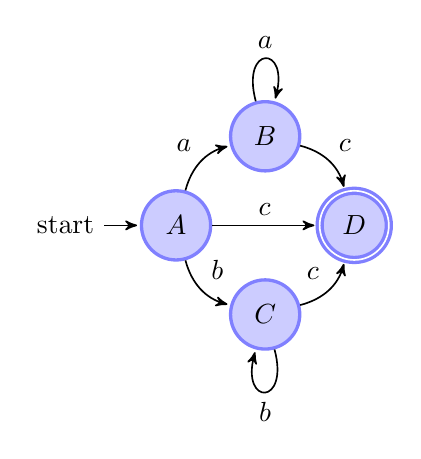
\begin{tikzpicture}[->,>=stealth',shorten >=1pt,auto,node distance=1.6cm,semithick]
  \tikzstyle{every state}=[draw=blue!50,very thick,fill=blue!20]

  \node[initial,state] 	(A)                   			 {$A$};
  % kleene(a)
  \node[state]		(B)	[above right of =A]	 {$B$};
  \node[state]		(C)	[below right of =A]	 {$C$};
    \node[state,accepting]		(D)	[above right of =C]	 {$D$};
 
		
  \path 			(A)	edge		[bend left]		node {$a$}	(B)
  					edge		[bend right]	node{$b$}	(C)
					edge					node{$c$}		(D)
				(B)	edge		[loop above]	node{$a$}	(B)
					edge		[bend left]		node{$c$}		(D)
				(C)	edge		[loop below]	node{$b$}	(C)
					edge		[bend right]	node{$c$}		(D);
\end{tikzpicture}
\end{center}



% (b$|$b)*abb(a$|$b)*
\subsection{2. (b$|$b)*abb(a$|$b)*}

\begin{center}
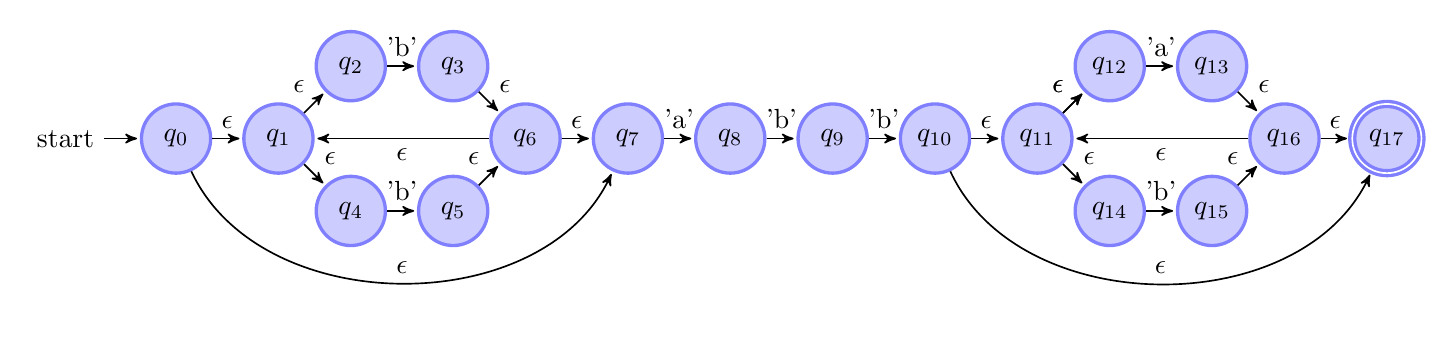
\begin{tikzpicture}[->,>=stealth',shorten >=1pt,auto,node distance=1.3cm,semithick]
  \tikzstyle{every state}=[draw=blue!50,very thick,fill=blue!20]

  \node[initial,state] 	(q0)                   			 			{$q_0$};
  \node[state]		(q1)		[right of=q0]	 			{$q_1$};
  \node[state]		(q2)		[above right of=q1]			 {$q_2$};
  \node[state]		(q3)		[right of=q2]				 {$q_3$};
  \node[state]		(q4)		[below right of=q1]			 {$q_4$};
  \node[state]		(q5)		[right of=q4]				 {$q_5$};
  \node[state]		(q6)		[below right of=q3]			 {$q_6$};
  \node[state]		(q7)		[right of=q6]				 {$q_7$};
  \node[state]		(q8)		[right of=q7]				 {$q_8$};
  \node[state]		(q9)		[right of=q8]				 {$q_9$};
  \node[state]		(q10)	[right of=q9]				 {$q_{10}$};
  \node[state]		(q11)	[right of=q10]				 {$q_{11}$};
  \node[state]		(q12)	[above right of=q11]		       	 {$q_{12}$};
  \node[state]		(q13)	[right of=q12]			       	 {$q_{13}$};
  \node[state]		(q14)	[below right of=q11]			 {$q_{14}$};
  \node[state]		(q15)	[right of=q14]			 	 {$q_{15}$};
  \node[state]		(q16)	[below right of=q13]	 	 	{$q_{16}$};
  \node[state,accepting]		(q17)	[right of=q16]	 	 		{$q_{17}$};
  
  
  \path 			(q0)	edge	 						node {$\epsilon$}	(q1)
  				(q0)	edge	 [bend right=65]			node {$\epsilon$}	(q7)
				(q1)	edge	 						node {$\epsilon$}	(q2)
				(q1)	edge	 						node {$\epsilon$}	(q4)
				(q2)	edge	 						node {'b'}			(q3)
				(q3)	edge	 						node {$\epsilon$}	(q6)
				(q6)	edge	 		 				node {$\epsilon$}	(q1)
				(q4)	edge	 		 				node {'b'}	(q5)
				(q5)	edge	 						node {$\epsilon$}	(q6)
				(q6)	edge	 						node {$\epsilon$}	(q7)
				(q7)	edge	 						node {'a'}	(q8)
				(q8)	edge	 						node {'b'}	(q9)
				(q9)	edge	 						node {'b'}	(q10)
				(q10)edge 			 			node {$\epsilon$}	(q11)
				(q10)edge [bend right=65]	 		node {$\epsilon$}	(q17)
				(q11)edge 			 			node {$\epsilon$}	(q12)
				(q11)edge 			 			node {$\epsilon$}	(q14)
				(q11)edge 			 			node {$\epsilon$}	(q12)
				(q12)edge 			 			node {'a'}	(q13)
				(q13)edge 			 			node {$\epsilon$}	(q16)
				(q16)edge 			 			node {$\epsilon$}	(q11)
				(q14)edge 			 			node {'b'}	(q15)
				(q15)edge 			 			node {$\epsilon$}	(q16)
				(q16)edge 			 			node {$\epsilon$}	(q17)
				;
\end{tikzpicture}
\end{center}


\subsection{3. (a$|$b)*a(a$|$b)(a$|$b)}

\begin{center}
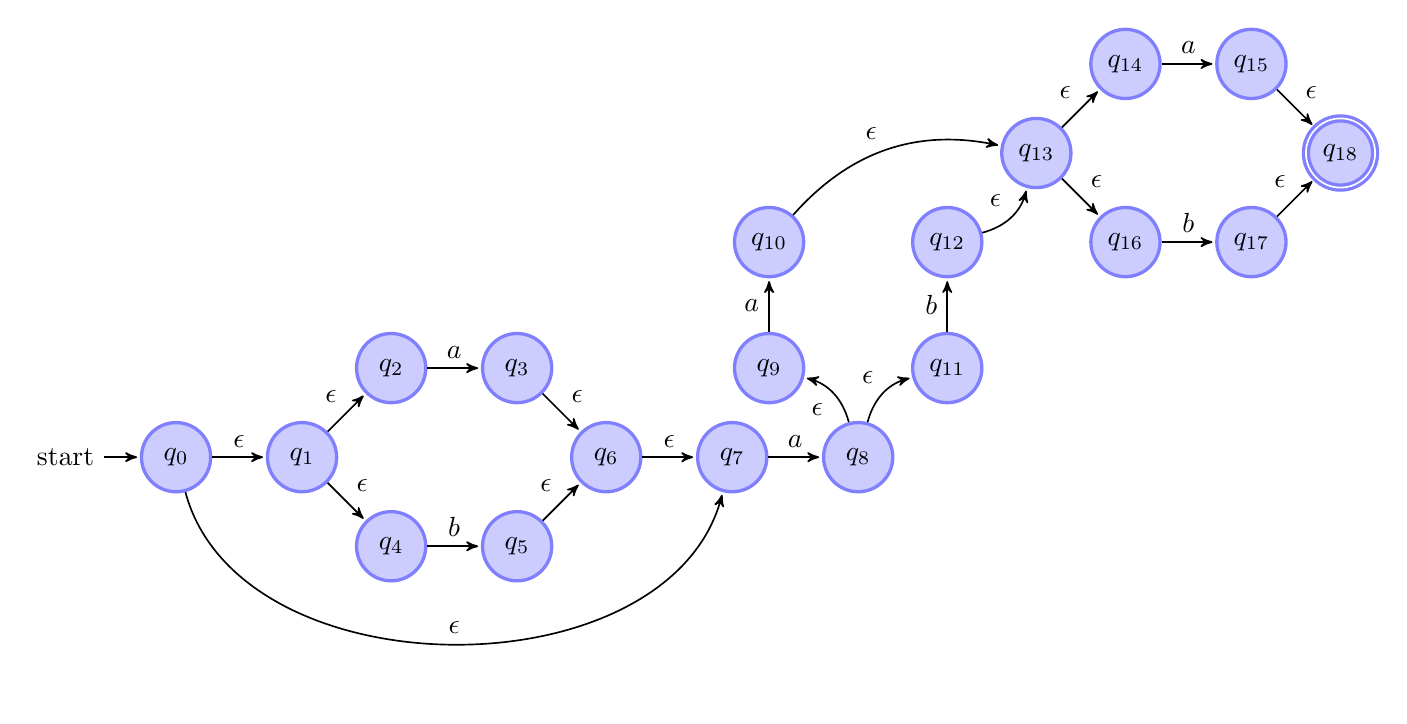
\begin{tikzpicture}[->,>=stealth',shorten >=1pt,auto,node distance=1.6cm,semithick]
  \tikzstyle{every state}=[draw=blue!50,very thick,fill=blue!20]

  \node[initial,state] 	(q0)                   			 {$q_0$};
  \node[state]		(q1) [right of=q0]                  			 {$q_1$};
  \node[state]		(q2) [above right of=q1]                  			 {$q_2$};
  \node[state]		(q3) [right of=q2]                  			 {$q_3$};
  \node[state]		(q4) [below right of=q1]                  			 {$q_4$};
  \node[state]		(q5) [right of=q4]                  			 {$q_5$};
  \node[state]		(q6)                 [below right of=q3]  			 {$q_6$};
  \node[state]		(q7)  [right of=q6]                			 {$q_7$};
  \node[state]		(q8)  [right of=q7]                 			 {$q_8$};
  \node[state]		(q9)  [above left of=q8]                 			 {$q_9$};
  \node[state]		(q10) [above of=q9]                  			 {$q_{10}$};
  \node[state]		(q11) [above right of=q8]                  			 {$q_{11}$};
  \node[state]		(q12)  [above of=q11]                 			 {$q_{12}$};
  \node[state]		(q13)  [above right of=q12]                 			 {$q_{13}$};
  \node[state]		(q14)  [above right of=q13]                 			 {$q_{14}$};
  \node[state]		(q15)  [right of=q14]                			 {$q_{15}$};
  \node[state]		(q16)  [below right of=q13]                 			 {$q_{16}$};
  \node[state]		(q17)  [right of=q16]                 			 {$q_{17}$};
  \node[state,accepting]		(q18)  [above right of=q17]                  			 {$q_{18}$};
		
  \path 			(q0)	edge			node {$\epsilon$}	(q1)
  				(q0)	edge		[bend right=75]		node {$\epsilon$}	(q7)
				(q1)	edge			node {$\epsilon$}	(q2)
				(q1)	edge			node {$\epsilon$}	(q4)
				(q2)	edge			node {$a$}	(q3)
				(q4)	edge			node {$b$}	(q5)
				(q3)	edge			node {$\epsilon$}	(q6)
				(q5)	edge			node {$\epsilon$}	(q6)
				(q6)	edge			node {$\epsilon$}	(q7)
				(q7)	edge			node {$a$}	(q8)
				(q8)	edge	 [bend right]		node {$\epsilon$}	(q9)
				(q8)	edge	 [bend left]		node {$\epsilon$}	(q11)
				(q9)	edge			node {$a$}	(q10)
				(q11)	edge			node {$b$}	(q12)
				(q10)	edge	 [bend left]		node {$\epsilon$}	(q13)
				(q12)	edge	 [bend right]		node {$\epsilon$}	(q13)
				(q13)	edge	 		node {$\epsilon$}	(q14)
				(q13)	edge	 	node {$\epsilon$}	(q16)
				(q14)	edge	 	node {$a$}	(q15)
				(q16)	edge	 	node {$b$}	(q17)
				(q15)	edge	 	node {$\epsilon$}	(q18)
				(q17)	edge	 	node {$\epsilon$}	(q18)
				
				
				;
\end{tikzpicture}
\end{center}


\subsection{4. b*ab? = b*a(b$| \epsilon$)}

\begin{center}
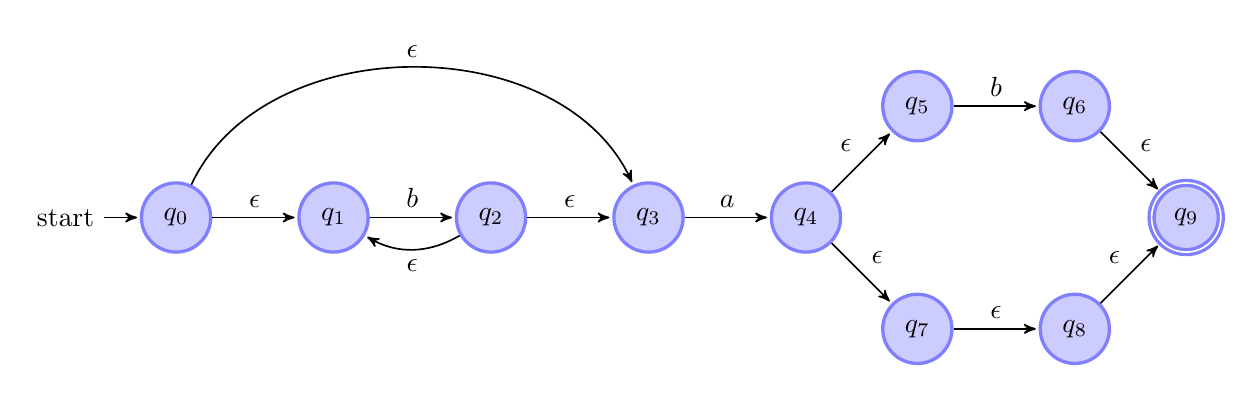
\begin{tikzpicture}[->,>=stealth',shorten >=1pt,auto,node distance=2cm,semithick]
  \tikzstyle{every state}=[draw=blue!50,very thick,fill=blue!20]

  \node[initial,state] 	(q0)                   			 {$q_0$};
  \node[state]		(q1) [right of=q0]                 			 {$q_1$};
  \node[state]		(q2) [right of=q1]                 			 {$q_2$};
  \node[state]		(q3) [right of=q2]                  			 {$q_3$};
  \node[state]		(q4) [right of=q3]                   			 {$q_4$};
  \node[state]		(q5) [above right of=q4]                   			 {$q_5$};
  \node[state]		(q6) [right of=q5]                  			 {$q_6$};
  \node[state]		(q7) [below right of=q4]                  			 {$q_7$};
  \node[state]		(q8) [right of=q7]                   			 {$q_8$};
  \node[state,accepting]		(q9) [above right of=q8]                   			 {$q_9$};
		
  \path 			(q0)	edge				node {$\epsilon$}	(q1)
  				(q0)	edge [bend left=65]				node {$\epsilon$}	(q3)
				(q1)	edge				node {$b$}	(q2)
				(q2)	edge	 [bend left]		node {$\epsilon$}	(q1)
				(q2)	edge				node {$\epsilon$}	(q3)
				(q3)	edge				node {$a$}	(q4)
				(q4)	edge				node {$\epsilon$}	(q5)
				(q4)	edge				node {$\epsilon$}	(q7)
				(q5)	edge				node {$b$}	(q6)
				(q7)	edge				node {$\epsilon$}	(q8)
				(q6)	edge				node {$\epsilon$}	(q9)
				(q8)	edge				node {$\epsilon$}	(q9)
							;
\end{tikzpicture}
\end{center}

\subsection{5. ab*ab*}

\begin{center}
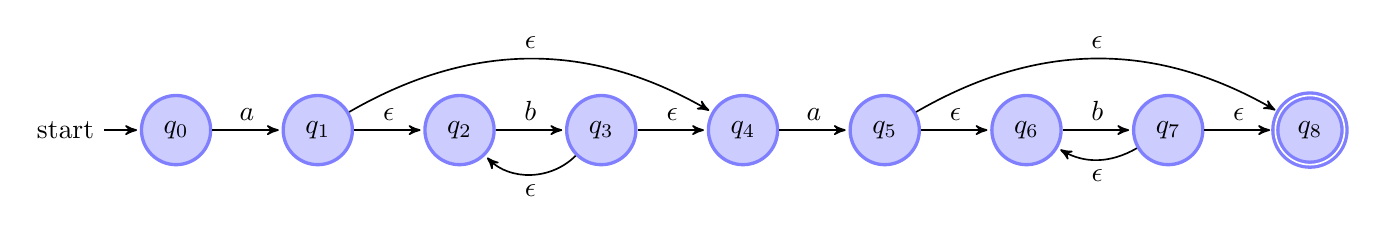
\begin{tikzpicture}[->,>=stealth',shorten >=1pt,auto,node distance=1.8cm,semithick]
  \tikzstyle{every state}=[draw=blue!50,very thick,fill=blue!20]

  \node[initial,state] 	(q0)                   			 {$q_0$};
  \node[state]				(q1) [right of=q0]                  			 {$q_1$};
\node[state]				(q2) [right of=q1]                  			 {$q_2$};
\node[state]				(q3) [right of=q2]                 			 {$q_3$};
\node[state]				(q4) [right of=q3]                 			 {$q_4$};
\node[state]				(q5) [right of=q4]                 			 {$q_5$};
\node[state]				(q6)  [right of=q5]                 			 {$q_6$};
\node[state]				(q7) [right of=q6]                  			 {$q_7$};
\node[state,accepting]				(q8) [right of=q7]                   			 {$q_8$};
		
  \path 			(q0)	edge			node {$a$}	(q1)
				(q1)	edge			node {$\epsilon$}	(q2)
				(q1)	edge	 [bend left]		node {$\epsilon $}	(q4)
				(q2)	edge				node {$b$}	(q3)
				(q3)	edge				node {$\epsilon$}	(q4)
				(q3)	edge	 [bend left=45]			node {$\epsilon$}	(q2)
				(q4)	edge			node {$a$}	(q5)
				(q5)	edge			node {$\epsilon$}	(q6)
				(q5)	edge	 [bend left]		node {$\epsilon$}	(q8)
				(q6)	edge			node {$b$}	(q7)
				(q7)	edge	 [bend left]		node {$\epsilon$}	(q6)
				(q7)	edge			node {$\epsilon$}	(q8)
				
				
					
				;
\end{tikzpicture}
\end{center}

\subsection{6. 0(0$|$1)*0}

\begin{center}
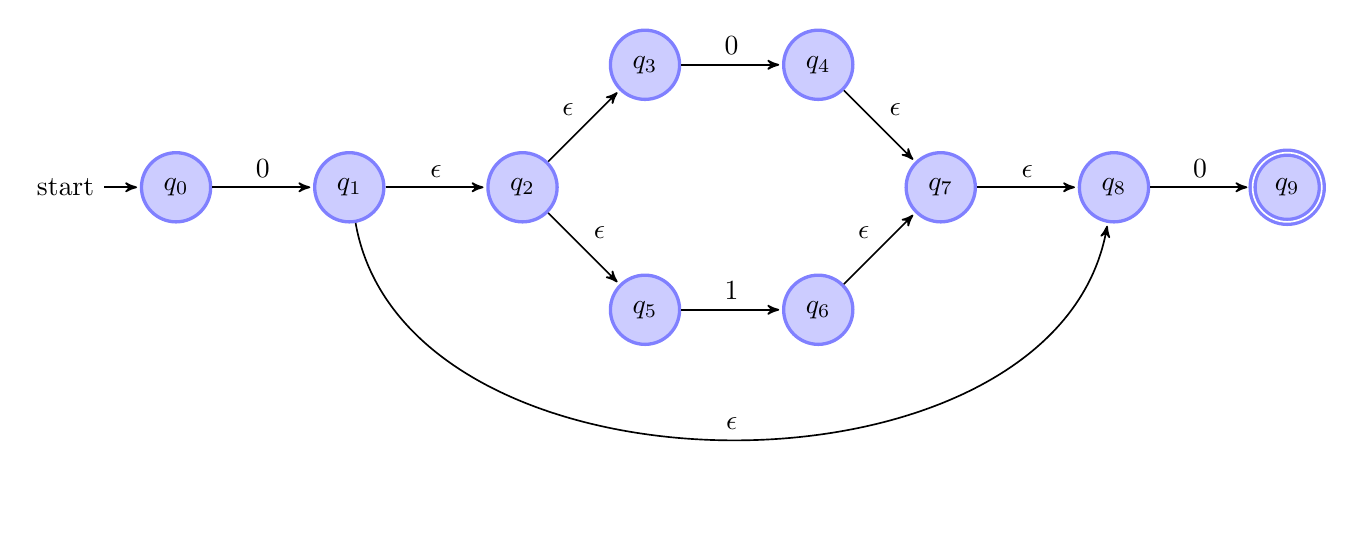
\begin{tikzpicture}[->,>=stealth',shorten >=1pt,auto,node distance=2.2cm,semithick]
  \tikzstyle{every state}=[draw=blue!50,very thick,fill=blue!20]

  \node[initial,state] 	(q0)                   			 {$q_0$};
  \node[state]		(q1)  [right of=q0]                 			 {$q_1$};
  \node[state]		(q2)  [right of=q1]                 			 {$q_2$};
  \node[state]		(q3)  [above right of=q2]                 			 {$q_3$};
  \node[state]		(q4) [right of=q3]                  			 {$q_4$};
  \node[state]		(q5) [below right of=q2]                  			 {$q_5$};
  \node[state]		(q6) [right of=q5]                  			 {$q_6$};
  \node[state]		(q7) [above right of=q6]                  			 {$q_7$};
  \node[state]		(q8) [right of=q7]                  			 {$q_8$};
  \node[state,accepting]		(q9) [right of=q8]                  			 {$q_9$};	
		
  \path 			(q0)	edge			node {$0$}	(q1)
  				(q1)	edge			node {$\epsilon$}	(q2)
				(q1)	edge		[bend right=80]		node {$\epsilon$}	(q8)
				
				(q2)	edge			node {$\epsilon$}	(q3)
				(q2)	edge			node {$\epsilon$}	(q5)
				(q4)	edge			node {$\epsilon$}	(q7)
				(q6)	edge			node {$\epsilon$}	(q7)
				(q7)	edge			node {$\epsilon$}	(q8)
				(q3)	edge			node {$0$}	(q4)
				(q5)	edge			node {$1$}	(q6)
				(q8)	edge			node {$0$}	(q9)
				;
\end{tikzpicture}
\end{center}


\subsection{7. (0$|$1)*0(0$|$1)(0$|$1)? = (0$|$1)*0(0$|$1)[(0$|$1)$| \epsilon$]}

\begin{center}
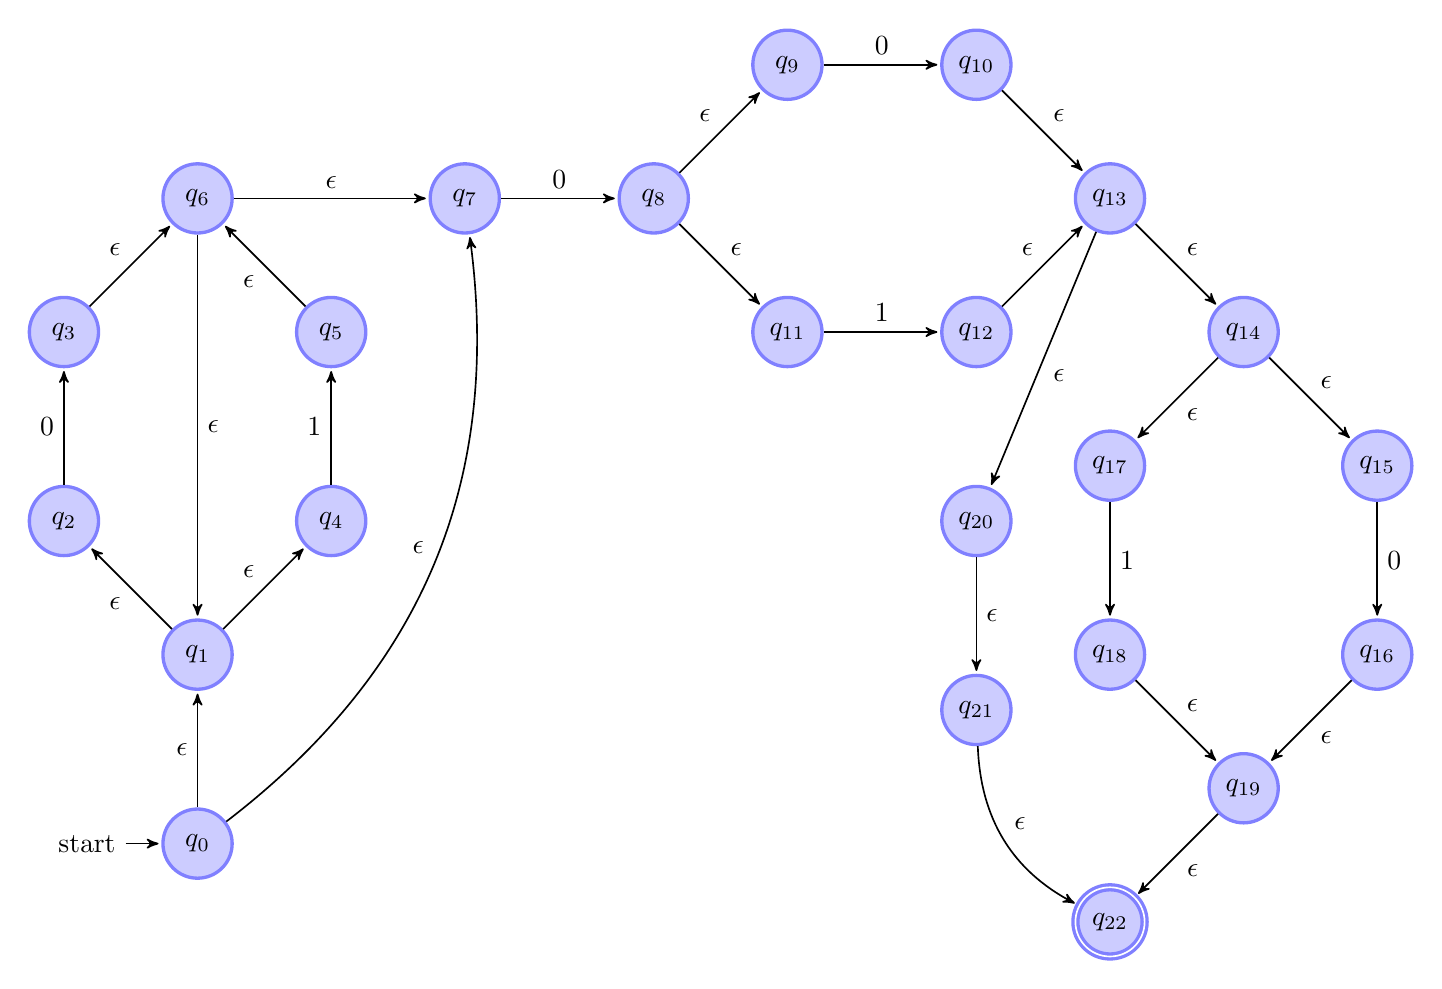
\begin{tikzpicture}[->,>=stealth',shorten >=1pt,auto,node distance=2.4cm,semithick]
  \tikzstyle{every state}=[draw=blue!50,very thick,fill=blue!20]

  \node[initial,state] 	(q0)                   			 {$q_0$};
  \node[state]		(q1)    [above of =q0]               			 {$q_1$};
  \node[state]		(q2)    [above left of=q1]               			 {$q_2$};
  \node[state]		(q3)   [above of =q2]                			 {$q_3$};
  \node[state]		(q4)   [above right of=q1]               			 {$q_4$};
  \node[state]		(q5)    [above of=q4]               			 {$q_5$};
  \node[state]		(q6)  [above left of=q5]                  			 {$q_6$};
  \node[state]		(q7)  [above right of=q5]                 			 {$q_7$};
  \node[state]		(q8)  [right of=q7]                 			 {$q_8$};
  \node[state]		(q9)   [above right of=q8]                			 {$q_9$};
  \node[state]		(q10)  [right of=q9]                			 {$q_{10}$};
  \node[state]		(q11)   [below right of=q8]                			 {$q_{11}$};
  \node[state]		(q12)   [right of=q11]                			 {$q_{12}$};
  \node[state]		(q13)  [above right of=q12]                 			 {$q_{13}$};
  \node[state]		(q14)   [below right of=q13]                			 {$q_{14}$};
  \node[state]		(q15)  [below right of =q14]                 			 {$q_{15}$};
  \node[state]		(q16)  [below of=q15]                 			 {$q_{16}$};
  \node[state]		(q17) [below  left of=q14]                			 {$q_{17}$};
  \node[state]		(q18)  [below of=q17]                 			 {$q_{18}$};
  \node[state]		(q19)   [below right of=q18]                			 {$q_{19}$};
  \node[state]		(q20)  [below of =q12]                 			 {$q_{20}$};
  \node[state]		(q21)  [below of=q20]                 			 {$q_{21}$};
  \node[state,accepting]		(q22) [below left of=q19]                   			 {$q_{22}$};
  		
  \path 			(q0)	edge			node {$\epsilon$}	(q1)
  					edge  [bend right]  node {$\epsilon$}	(q7)
				(q1)	edge			node {$\epsilon$}	(q2)
				(q1)	edge			node {$\epsilon$}	(q4)
				(q3)	edge			node {$\epsilon$}	(q6)
				(q5)	edge			node {$\epsilon$}	(q6)
				(q6)	edge			node {$\epsilon$}	(q7)
				(q7)	edge			node {$0$}	(q8)
				(q8)	edge			node {$\epsilon$}	(q9)
				(q8)	edge			node {$\epsilon$}	(q11)
				(q10)	edge			node {$\epsilon$}	(q13)
				(q12)	edge			node {$\epsilon$}	(q13)
				(q13)	edge			node {$\epsilon$}	(q14)
				(q13)	edge			node {$\epsilon$}	(q20)
				(q2)	edge			node {$0$}	(q3)
				(q4)	edge			node {$1$}	(q5)
				(q9)	edge			node {$0$}	(q10)
				(q11)	edge			node {$1$}	(q12)
				(q14)	edge			node {$\epsilon$}	(q15)
				(q14)	edge			node {$\epsilon$}	(q17)
				(q16)	edge			node {$\epsilon$}	(q19)
				(q18)	edge			node {$\epsilon$}	(q19)
				(q21)	edge	 [bend right]		node {$\epsilon$}	(q22)
				(q19)	edge			node {$\epsilon$}	(q22)
				(q20)	edge			node {$\epsilon$}	(q21)
				(q17)	edge			node {$1$}	(q18)
				(q15)	edge			node {$0$}	(q16)
				(q6)	edge 		node {$\epsilon$}	(q1)
				;
\end{tikzpicture}
\end{center}

\subsection{8. (0$|$1)1*(0$|$1)}

\begin{center}
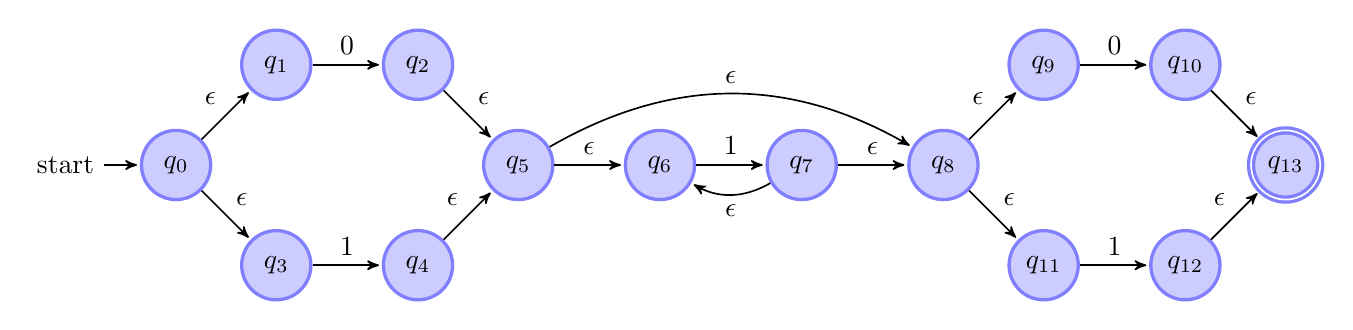
\begin{tikzpicture}[->,>=stealth',shorten >=1pt,auto,node distance=1.8cm,semithick]
  \tikzstyle{every state}=[draw=blue!50,very thick,fill=blue!20]

  \node[initial,state] 	(q0)                   			 {$q_0$};
  \node[state]		(q1)  [above right of=q0]                 			 {$q_1$};
  \node[state]		(q2)  [right of=q1]                 			 {$q_2$};
  \node[state]		(q3)  [below right of=q0]                 			 {$q_3$};
  \node[state]		(q4)   [right of=q3]                			 {$q_4$};
  \node[state]		(q5)   [above right of=q4]                			 {$q_5$};
  \node[state]		(q6)  [right of=q5]                 			 {$q_6$};
  \node[state]		(q7)   [right of=q6]                			 {$q_7$};
  \node[state]		(q8)    [right of=q7]               			 {$q_8$};
  \node[state]		(q9)    [above right of=q8]               			 {$q_9$};
  \node[state]		(q10)  [right of=q9]                 			 {$q_{10}$};
  \node[state]		(q11)   [below right of=q8]                			 {$q_{11}$};
  \node[state]		(q12)  [right of=q11]                 			 {$q_{12}$};
  \node[state,accepting]		(q13) [above right of=q12]                   			 {$q_{13}$};	
		
  \path 			(q0)	edge			node {$\epsilon$}	(q1)
				(q0)	edge				node {$\epsilon$}	(q3)
				(q4)	edge				node {$\epsilon$}	(q5)
				(q2)	edge				node {$\epsilon$}	(q5)
				(q7)	edge	 [bend left]			node {$\epsilon$}	(q6)
				(q5)	edge [bend left]				node {$\epsilon$}	(q8)
				(q8)	edge				node {$\epsilon$}	(q9)
				(q8)	edge				node {$\epsilon$}	(q11)
				(q10)	edge				node {$\epsilon$}	(q13)
				(q12)	edge				node {$\epsilon$}	(q13)
				(q1)	edge				node {$0$}	(q2)
				(q3)	edge				node {$1$}	(q4)
				(q5)	edge				node {$\epsilon$}	(q6)
				(q6)	edge				node {$1$}	(q7)
				(q9)	edge				node {$0$}	(q10)
				(q11)	edge				node {$1$}	(q12)
				(q7)	edge				node {$\epsilon$}	(q8)
				;
\end{tikzpicture}
\end{center}


\subsection{9. 0?(1$| \epsilon$)?0* = (0$| \epsilon$) [ (1$| \epsilon$) $| \epsilon$ )] 0*))}

\begin{center}
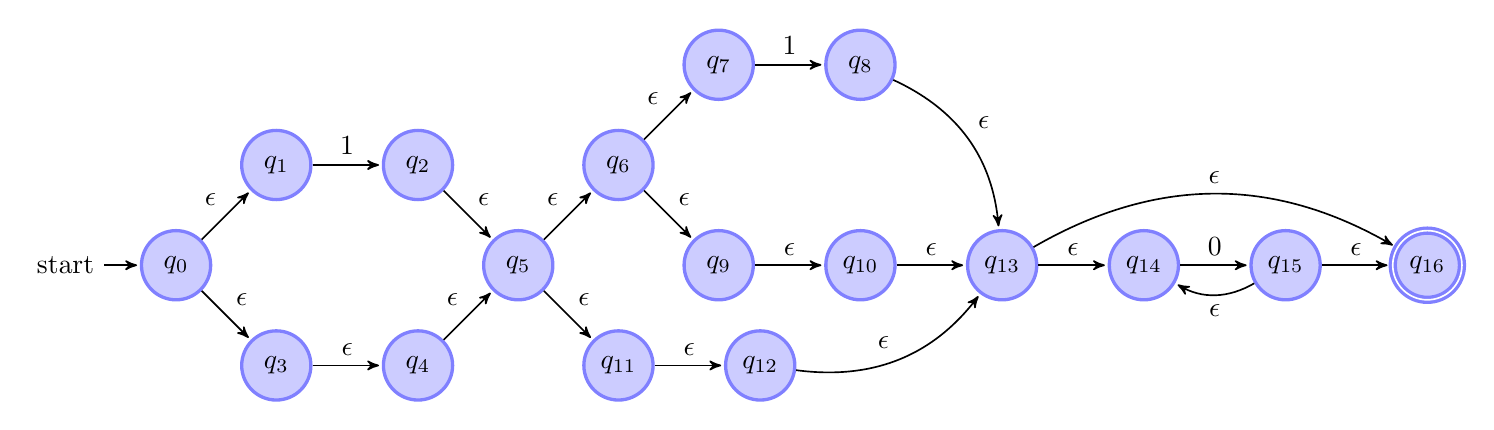
\begin{tikzpicture}[->,>=stealth',shorten >=1pt,auto,node distance=1.8cm,semithick]
  \tikzstyle{every state}=[draw=blue!50,very thick,fill=blue!20]

  \node[initial,state] 	(q0)                   			 {$q_0$};
  \node[state]		(q1) [above right of=q0]                   			 {$q_1$};
  \node[state]		(q2) [right of=q1]                   			 {$q_2$};
  \node[state]		(q3)  [below right of=q0]                 			 {$q_3$};
  \node[state]		(q4)  [right of=q3]                 			 {$q_4$};
  \node[state]		(q5) [above right of=q4]                   			 {$q_5$};
  \node[state]		(q6) [above right of=q5]                 			 {$q_6$};
  \node[state]		(q7) [above right of=q6]                  			 {$q_7$};
  \node[state]		(q8) [right of=q7]                  			 {$q_8$};
  \node[state]		(q9) [below right of=q6]                  			 {$q_9$};
  \node[state]		(q10)  [right of=q9]                 			 {$q_{10}$};
  \node[state]		(q11)  [below right of=q5]                 			 {$q_{11}$};
  \node[state]		(q12) [right of=q11]                  			 {$q_{12}$};
  \node[state]		(q13)  [right of=q10]                 			 {$q_{13}$};
  \node[state]		(q14)  [right of=q13]                  			 {$q_{14}$};
  \node[state]		(q15) [right of=q14]                  			 {$q_{15}$};
  \node[state,accepting]		(q16) [right of=q15]                   			 {$q_{16}$};
		
  \path 			(q0)	edge			node {$\epsilon$}	(q1)
  				(q0)	edge			node {$\epsilon$}	(q3)
				(q3)	edge			node {$\epsilon$}	(q4)
				(q4)	edge			node {$\epsilon$}	(q5)
				(q2)	edge			node {$\epsilon$}	(q5)
				(q5)	edge			node {$\epsilon$}	(q6)
				(q5)	edge			node {$\epsilon$}	(q11)
				(q6)	edge			node {$\epsilon$}	(q7)
				(q6)	edge			node {$\epsilon$}	(q9)
				(q9)	edge			node {$\epsilon$}	(q10)
				(q8)	edge	 [bend left]		node {$\epsilon$}	(q13)
				(q10)	edge			node {$\epsilon$}	(q13)
				(q12)	edge	 [bend right]		node {$\epsilon$}	(q13)
				(q7)	edge			node {$1$}	(q8)
				(q13)	edge			node {$\epsilon$}	(q14)
				(q1)	edge			node {$1$}	(q2)
				(q14)	edge			node {$0$}	(q15)
				(q13)	edge	 [bend left]		node {$\epsilon$}	(q16)
				(q11)	edge			node {$\epsilon$}	(q12)
				(q15)	edge			node {$\epsilon$}	(q16)
				(q15)	edge	 [bend left]		node {$\epsilon$}	(q14)
  
				;
\end{tikzpicture}
\end{center}

\subsection{10. (01)*(10)*)}

\begin{center}
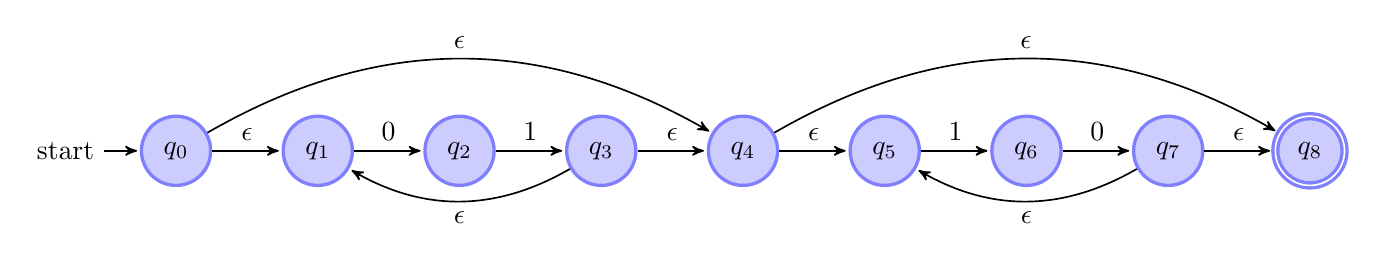
\begin{tikzpicture}[->,>=stealth',shorten >=1pt,auto,node distance=1.8cm,semithick]
  \tikzstyle{every state}=[draw=blue!50,very thick,fill=blue!20]

  \node[initial,state] 	(q0)                   			 {$q_0$};
  \node[state]		(q1) [right of=q0]                  			 {$q_1$};
  \node[state]		(q2) [right of=q1]                  			 {$q_2$};
  \node[state]		(q3)  [right of=q2]                 			 {$q_3$};
  \node[state]		(q4) [right of=q3]                  			 {$q_4$};
  \node[state]		(q5) [right of=q4]                  			 {$q_5$};
  \node[state]		(q6) [right of=q5]                  			 {$q_6$};
  \node[state]		(q7) [right of=q6]                  			 {$q_7$};
  \node[state,accepting] (q8)        [right of=q7]           			 {$q_8$};  
		
  \path 			(q0)	edge		node {$\epsilon$}	(q1)
				  (q0)	edge	 [bend left]	node {$\epsilon$}	(q4)
				(q1)	edge		node {$0$}	(q2)
				(q2)	edge		node {$1$}	(q3)
				(q3)	edge		node {$\epsilon$}	(q4)
				(q3)	edge	 [bend left]	node {$\epsilon$}	(q1)
				(q4)	edge		node {$\epsilon$}	(q5)
				(q5)	edge		node {$1$}	(q6)
				(q6)	edge		node {$0$}	(q7)
				(q7)	edge		node {$\epsilon$}	(q8)
				(q7)	edge	[bend left]	node {$\epsilon$}	(q5)
				(q4)	edge	[bend left]	node {$\epsilon$}	(q8);
\end{tikzpicture}
\end{center}

\end{homeworkProblem}

\section{Demuestre que $L(r$*$) = L(r|\epsilon)$}

Tomemos el Automata No-determinista que acepta al lenguaje denotado por r*

\begin{center}
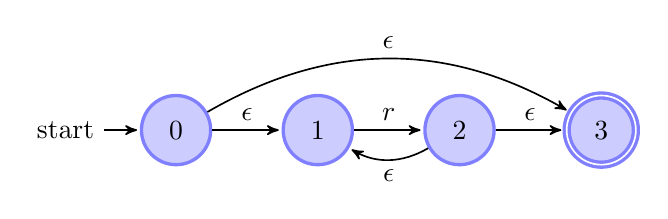
\begin{tikzpicture}[->,>=stealth',shorten >=1pt,auto,node distance=1.8cm,semithick]
  \tikzstyle{every state}=[draw=blue!50,very thick,fill=blue!20]

  \node[initial,state] 	(q0)                   			 {$0$};
  \node[state]		(q1) [right of=q0]                  			 {$1$};
  \node[state]		(q2) [right of=q1]                  			 {$2$};
  \node[state,accepting]		(q3)  [right of=q2]                 			 {$3$};
  
		
  \path 			(q0)	edge		node {$\epsilon$}	(q1)
				(q0)	edge	 [bend left]	node {$\epsilon$}	(q3)
				(q1)	edge		node {$r$}	(q2)
				(q2)	edge	 [bend left] 	node {$\epsilon$}	(q1)
				(q2) edge 		node{$\epsilon$} (q3)
				;
\end{tikzpicture}
\end{center}
Apliquemos el algoritmo de construcci\'{o}n de sub-conjuntos y veamos que: \\

$q_0 = \cerradura{q_0} = A $ \\
$F_d = \set{}$ \\
$Q = \set{A}$\\
\indent $marcados = \set{A}$\\ 
\indent \indent para 'r' \\
\indent \indent \indent $U = \cerradura{mover(A,r)} = \cerradura{2} = \set{2,1,3} = B$\\
\indent \indent \indent $Q = \set{A,B}$
\indent \indent \indent $\delta = \set{(A,r) -> B}$\\

\indent $marcados = \set {A,B}$\\
\indent \indent para 'r'\\
\indent \indent \indent $U = \cerradura{mover(B,r)} = \cerradura{2} = \set{2,1,3} = B$\\
\indent \indent \indent $\delta = \set{(A,r) -> B,(B,r) -> B}$\\

$A \cap F_n \neq \emptyset$ \\
\indent $F_d = \set{A}$
$B \cap F_n \neq \emptyset$ \\
\indent $F_d = \set{A,B}$

tenemos un nuevo $DFA_1$ que tambi\'{e}n acepta a el lenguaje denotado por r*

\begin{center}
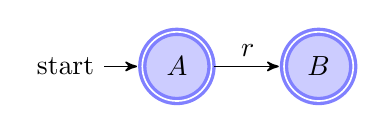
\begin{tikzpicture}[->,>=stealth',shorten >=1pt,auto,node distance=1.8cm,semithick]
  \tikzstyle{every state}=[draw=blue!50,very thick,fill=blue!20]

  \node[initial,state,accepting] 	(A)                   			 {$A$};
  \node[state,accepting]		(B) [right of=A]                  			 {$B$};
  
  \path 			(A)	edge		node {$r$}	(B)
				;
\end{tikzpicture}
\end{center}

Tomemos ahora el Automata No-Determinista que acepta al lenguaje denotado por la expresi\'{o}n regular r$| \epsilon$ 

\begin{center}
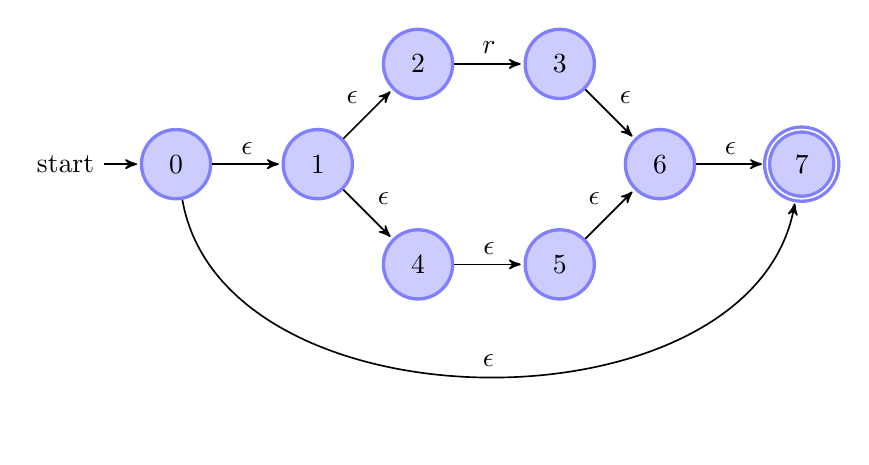
\begin{tikzpicture}[->,>=stealth',shorten >=1pt,auto,node distance=1.8cm,semithick]
  \tikzstyle{every state}=[draw=blue!50,very thick,fill=blue!20]

  \node[initial,state] 	(q0)                   			 {$0$};
  \node[state]		(q1) [right of=q0]                  			 {$1$};
  \node[state]		(q2) [above right of=q1]                  			 {$2$};
  \node[state]		(q3) [right of=q2]                  			 {$3$};
  \node[state]		(q4) [below right of=q1]                  			 {$4$};
  \node[state]		(q5) [right of=q4]                  			 {$5$};
  \node[state]		(q6) [above right of=q5]                  			 {$6$};
  \node[state,accepting]		(q7) [right of=q6]                  			 {$7$};
  
		
  \path 			(q0)	edge		node {$\epsilon$}	(q1)
  				(q0)	edge	 [bend right=80] 	node {$\epsilon$}	(q7)
				(q1)	edge		node {$\epsilon$}	(q2)
				(q1)	edge		node {$\epsilon$}	(q4)
				(q3)	edge		node {$\epsilon$}	(q6)
				(q5)	edge		node {$\epsilon$}	(q6)
				(q4)	edge		node {$\epsilon$}	(q5)
				(q2)	edge		node {$r$}	(q3)
				(q6)	edge		node {$\epsilon$}	(q7)				
				;
\end{tikzpicture}
\end{center}

Apliquemos entonces, el algoritmo de Construcci\'{o}n de subconjuntos 

$q_0 = \cerradura{0} = \set{0,1,2,4,5,6,7} = A $\\
$Q = \set{A}$

\indent $marcados = \set{A}$
\indent \indent para r \\
\indent \indent \indent $U = \cerradura{mueve(A,r)} = \cerradura{3} = \set{3,6,1,4,5,7} = B$\\
\indent \indent \indent $Q = \set{A,B}$\\
\indent \indent \indent $\delta = \set{(A,r) -> B}$\\

\indent $marcados = \set{B}$\\
\indent \indent para r\\
\indent \indent \indent $U = \cerradura{mueve(B,r)} = \cerradura{3} = \set{3,6,1,4,5,7} = B$\\
\indent \indent \indent $\delta = \set{(A,r) -> B, (B,r) -> B}$\\

$A \cap F_n \neq \emptyset$ \\
\indent $F_d = \set{A}$\\
$B \cap F_n \neq \emptyset$ \\
\indent $F_d = \set{A,B}$\\

tenemos ahora a un nuevo $DFA_2$ equivalente al NFA anterior. Notemos que este es isomorfo con $DFA_1$ por lo que aceptan al mismo lenguaje y son equivalentes. Por lo tanto, $L(r$*$) = L(r|\epsilon)$.

\begin{center}
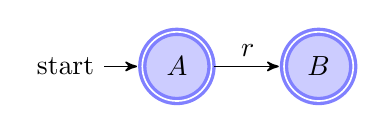
\begin{tikzpicture}[->,>=stealth',shorten >=1pt,auto,node distance=1.8cm,semithick]
  \tikzstyle{every state}=[draw=blue!50,very thick,fill=blue!20]

  \node[initial,state,accepting] 	(A)                   			 {$A$};
  \node[state,accepting]		(B) [right of=A]                  			 {$B$};
  
  \path 			(A)	edge		node {$r$}	(B)
				;
\end{tikzpicture}
\end{center}



 
\subsection{Bibliograf\'{i}a}


\end{spacing}
\end{document}

%%%%%%%%%%%%%%%%%%%%%%%%%%%%%%%%%%%%%%%%%%%%%%%%%%%%%%%%%%%%%
